%! Author = maxx
%! Date = 11/27/24

% Preamble
\documentclass[12pt]{report}

\usepackage[a4paper, left=2.5cm, right=2.5cm, top=3cm, bottom=3cm]{geometry}
\usepackage{graphicx}
\usepackage{pdfpages}
\usepackage{glossaries}
\usepackage{titling}
\setlength{\parindent}{0pt}


\title{POO - Laboratoire 7 \\ \large Calculatrice}
\author{Lestiboudois Maxime \& Parisod Nathan}
\date{27/11/2024}

% Redéfinir \maketitle pour inclure l'image sous le titre
\pretitle{\begin{center}\Huge\bfseries}
\posttitle{\par\end{center}\vspace{0.5cm}
\begin{center}

\includegraphics[scale = 0.2]{images/SingeCalculatrice}
\end{center}\vspace{0.5cm}}

% Document
\begin{document}
    \maketitle
    \tableofcontents
    \newpage

%%%%%%%%%%%%%%%%%%%%
%%  Introduction  %%
%%%%%%%%%%%%%%%%%%%%

    \section*{Introduction}
    \addcontentsline{toc}{section}{Introduction}
%%%%%%%%%%%%%%%%%%%%
%Cahier des charges%
%%%%%%%%%%%%%%%%%%%%
    \section*{Cahier des charges}
    \addcontentsline{toc}{section}{Cahier des charges}
        \subsection*{1. Objectif du Projet}
        \addcontentsline{toc}{subsection}{1. Objectif du Projet}
        Créer une calculatrice fonctionnant en notation polonaise inverse (Reverse Polish Notation - RPN). Elle doit inclure une interface graphique (GUI) et un mode console, réutilisant les mêmes classes et principes. Le projet doit suivre une architecture Modèle-Vue-Contrôleur (MVC).

        \subsection*{2. Spécifications Fonctionnelles}
        \addcontentsline{toc}{subsection}{2. Spécifications Fonctionnelles}
            \subsubsection*{2.1 Interface Graphique (GUI)}
            \addcontentsline{toc}{subsubsection}{2.1 Interface Graphique (GUI)}
                \begin{itemize}
                    \item Implémenter une interface utilisateur dans la classe JCalculator.
                    \item Boutons requis :
                    \begin{itemize}
                        \item Chiffres : 0-9.
                        \item Opérations unaires : sqrt, 1/x, \verb|x^2|.
                        \item Opérations binaires : +, -, *, /.
                        \item Autres boutons :
                        \begin{itemize}
                            \item MR : récupérer une valeur en mémoire.
                            \item MS : stocker une valeur en mémoire.
                            \item \verb|<=| : backspace pour supprimer le dernier caractère.
                            \item CE : réinitialiser l’affichage.
                            \item C : réinitialiser l’affichage et vider la pile.
                            \item Ent : placer la valeur courante sur la pile.
                            \item +/- : changer le signe de la valeur courante.
                            \item . : pour les nombres décimaux.
                        \end{itemize}
                    \end{itemize}

                    \item Affichage :
                    \begin{itemize}
                        \item Zone de texte (JTextField) pour la valeur courante.
                        \item Liste (JList) pour visualiser la pile.
                    \end{itemize}

                    \item Mise à jour de l'affichage après chaque opération via une méthode update().
                \end{itemize}
            \subsection*{2.2 Mode Console}
            \addcontentsline{toc}{subsection}{2.2 Mode Console}
                \begin{itemize}
                    \item Développer une classe Calculator permettant une interaction textuelle.
                    \item Commandes utilisateur :
                    \begin{itemize}
                        \item Saisir un nombre pour l’ajouter à la pile.
                        \item Entrer une opération (+, sqrt, etc.).
                        \item exit : quitter la calculatrice.
                    \end{itemize}

                    \item Fonctionnalités similaires à la version graphique :
                    \begin{itemize}
                        \item Gestion de la pile.
                        \item Support des opérations unaires, binaires et de mémoire.
                    \end{itemize}
                \end{itemize}

            \subsection*{2.3 Gestion des Données et Opérations}
            \addcontentsline{toc}{subsection}{2.3 Gestion des Données et Opérations}
                \begin{itemize}
                    \item Pile personnalisée (Stack) :
                    \begin{itemize}
                        \item Empiler une valeur.
                        \item Désempiler une valeur.
                        \item Obtenir l’état actuel de la pile sous forme de tableau.
                        \item Fournir un itérateur pour parcourir la pile.
                        \item Implémentée avec une liste chaînée sans structures Java préconstruites.
                    \end{itemize}

                    \item État interne (State) :
                    \begin{itemize}
                        \item Stocker :
                        \begin{itemize}
                            \item Valeur courante.
                            \item Pile des valeurs.
                            \item État d’erreur.
                        \end{itemize}

                        \item Fournir des méthodes pour gérer et manipuler ces données.
                    \end{itemize}
                \end{itemize}

            \subsection*{3. Spécifications Techniques}
            \addcontentsline{toc}{subsection}{3. Spécifications Techniques}
                \subsubsection*{3.1 Architecture MVC}
                \addcontentsline{toc}{subsubsection}{3.1 Architexture MVC}
                    \begin{itemize}
                        \item Modèle (State) :
                        \begin{itemize}
                            \item Indépendant de l’interface graphique.
                            \item Stocke les données et implémente la logique de calcul.
                        \end{itemize}

                        \item Vue (JCalculator) :
                        \begin{itemize}
                            \item Interface utilisateur graphique basée sur Swing.
                            \item Réagit aux changements dans le modèle.
                        \end{itemize}

                        \item Contrôleurs (Operator) :
                        \begin{itemize}
                            \item Boutons dans l’interface graphique agissant comme des contrôleurs.
                            \item Appel de la méthode execute() d’un objet Operator.
                        \end{itemize}
                    \end{itemize}
                \subsubsection*{3.2 Hiérarchie des Classes}
                \addcontentsline{toc}{subsubsection}{3.2 Hiérarchie des Classes}
                    \begin{itemize}
                        \item Classe générique Stack pour représenter une pile.
                        \item Classe State pour l'état interne.
                        \item Hiérarchie Operator :
                        \begin{itemize}
                            \item Classe de base Operator :
                            \begin{itemize}
                                \item Méthode execute().
                            \end{itemize}

                            \item Sous-classes spécialisées :
                            \begin{itemize}
                                \item NumberOperator, AdditionOperator, SqrtOperator, etc.
                            \end{itemize}
                        \end{itemize}

                        \item Classe JCalculator pour l'interface graphique.
                        \item Classe Calculator pour le mode console.
                    \end{itemize}
            \subsection*{4. Contraintes}
            \addcontentsline{toc}{subsection}{4. Contraintes}
                \begin{itemize}
                    \item Aucune utilisation de switch ou de if pour sélectionner l'opération dans Operator.
                    \item Pas de propriétés statiques pour le stockage des données.
                    \item Le code doit être modulaire et réutilisable.
                    \item Respect des principes de conception objet.
                \end{itemize}
            \subsection*{5. Tests}
            \addcontentsline{toc}{subsection}{5. Tests}
                \begin{itemize}
                    \item Élaborer une grille de tests couvrant :
                    \begin{itemize}
                        \item Les opérations unaires et binaires.
                        \item Les erreurs (ex. : division par zéro, pile vide).
                        \item Le stockage et rappel de mémoire.
                        \item La compatibilité entre le mode console et GUI.
                    \end{itemize}

                    \item Inclure des cas limites et des tests d'intégration.
                \end{itemize}
%%%%%%%%%%%%%%%%%%%%
%%  Schéma UML  %%
%%%%%%%%%%%%%%%%%%%%
    \section*{Schéma UML}
    \addcontentsline{toc}{section}{Schéma UML}
    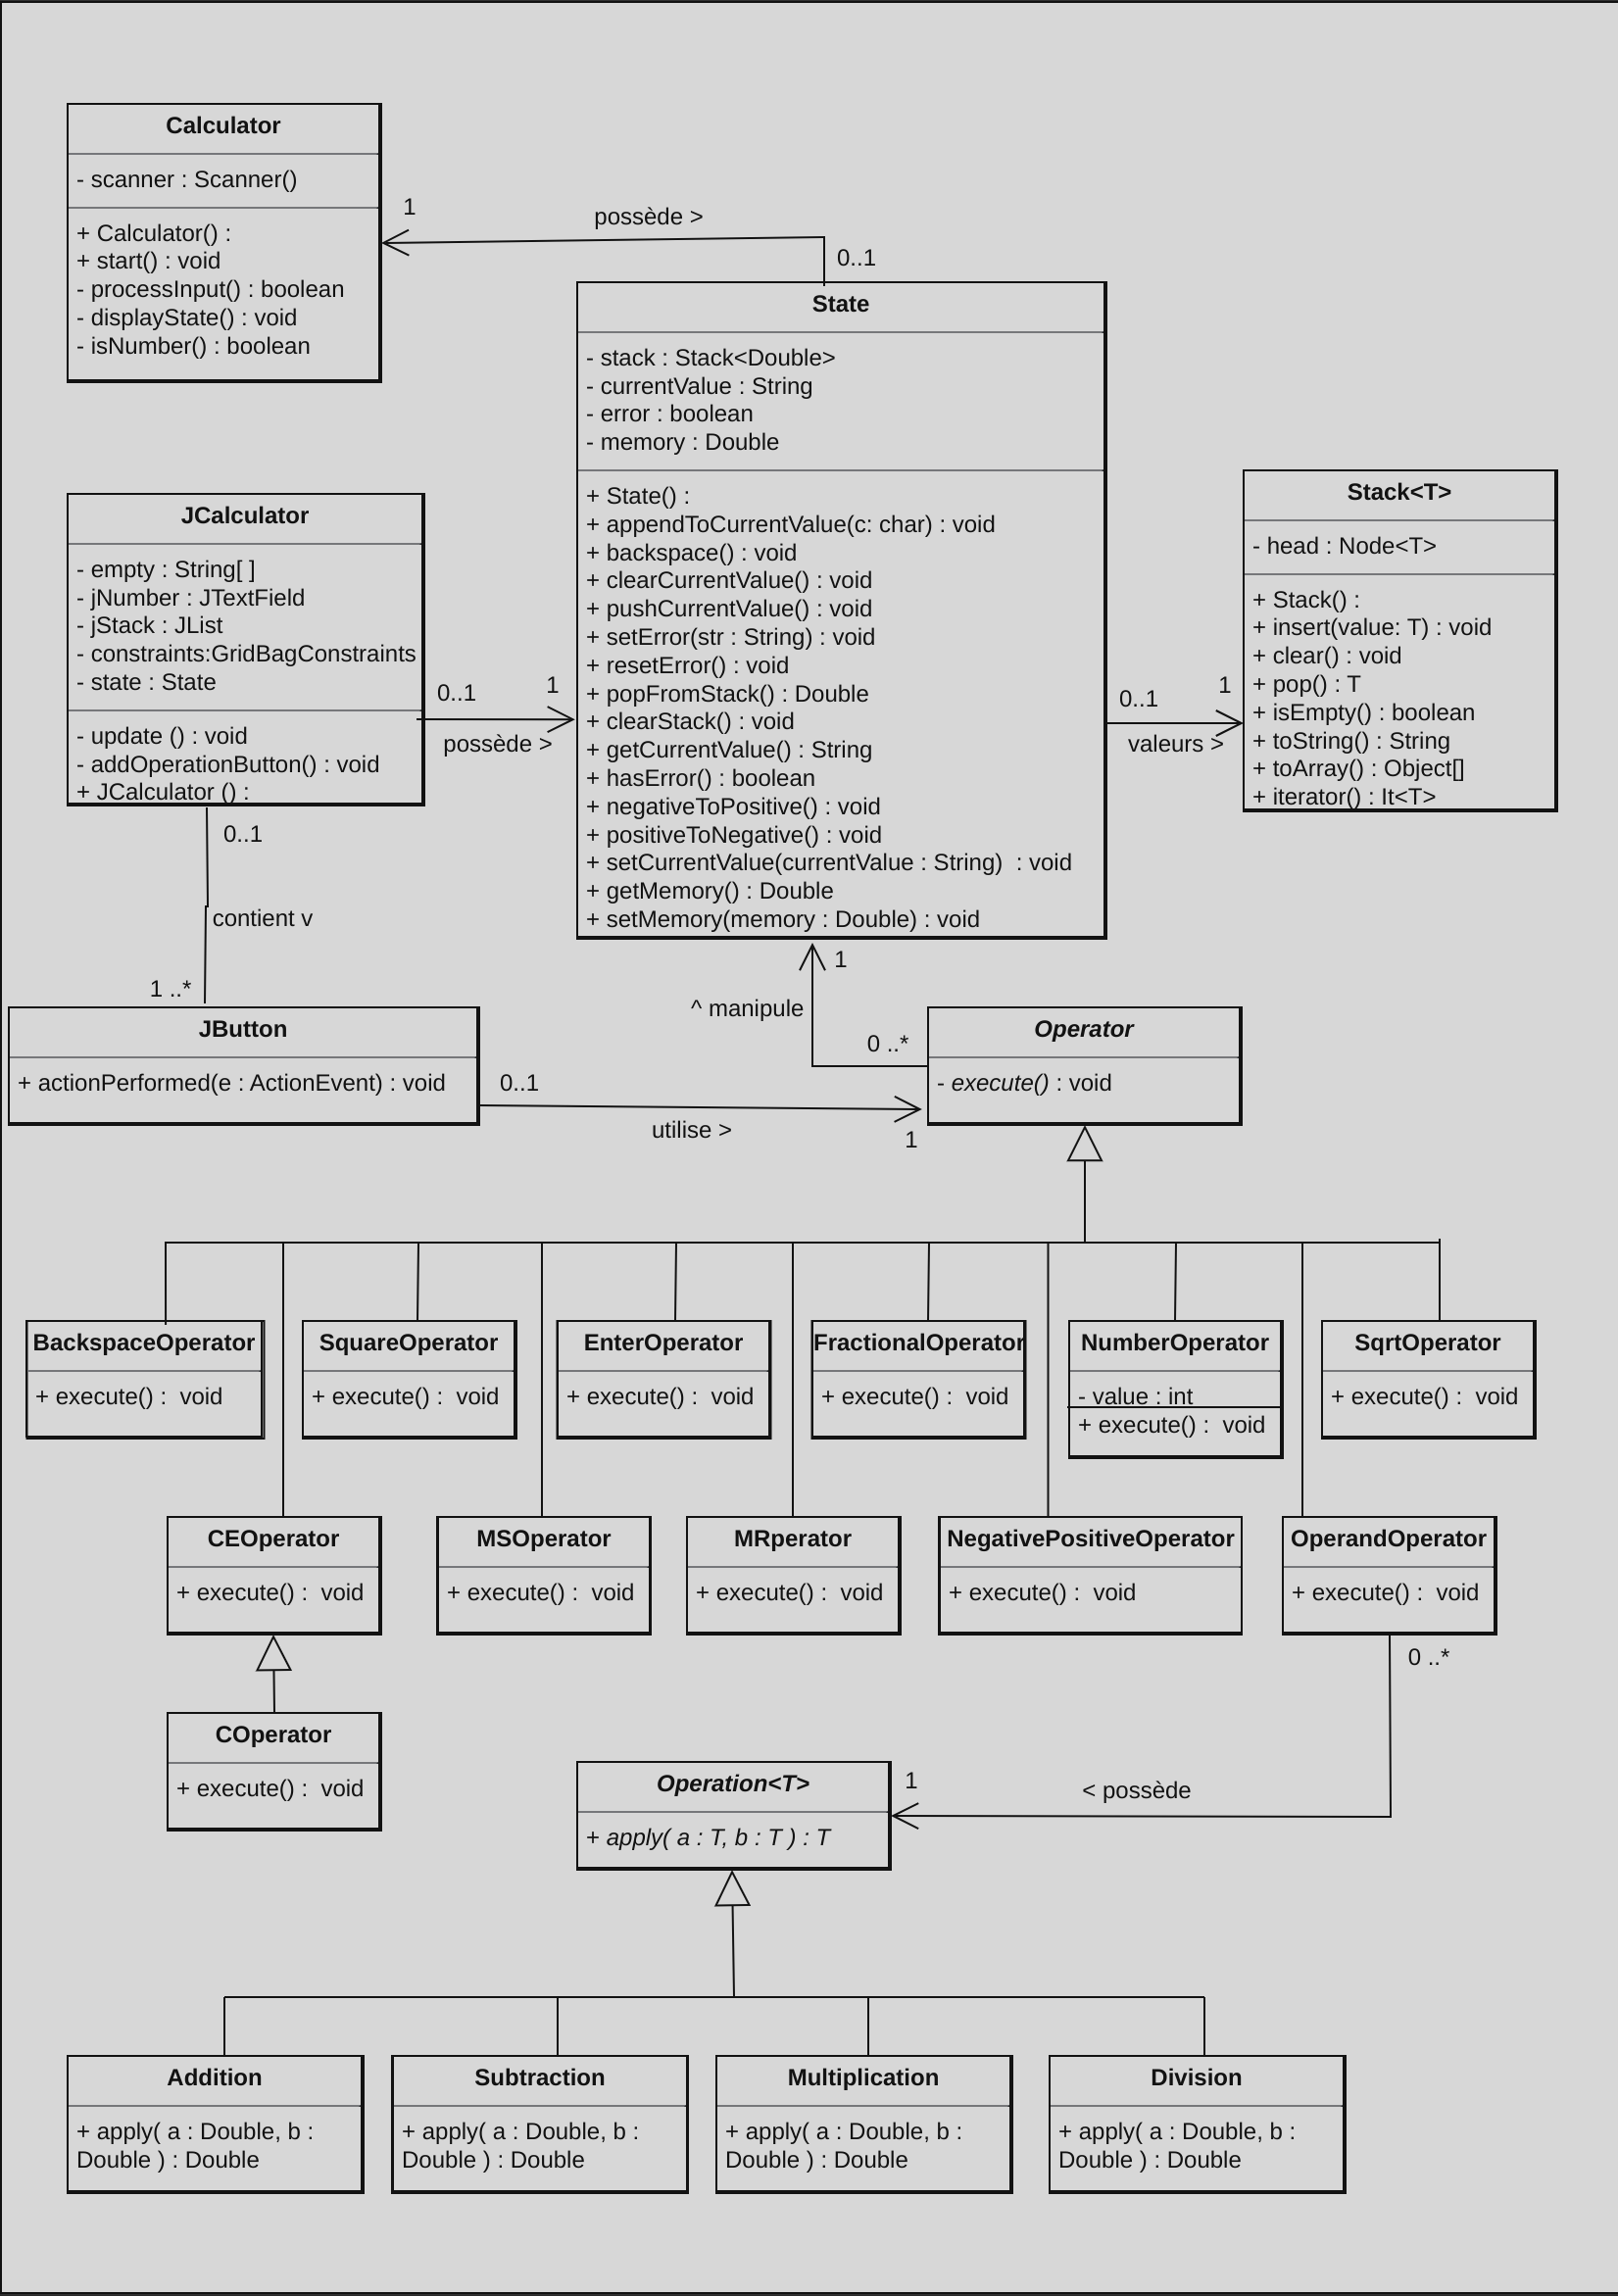
\includegraphics[scale=0.3]{images/diagram}
%%%%%%%%%%%%%%%%%%%%
%%  Listing code  %%
%%%%%%%%%%%%%%%%%%%%
    \section*{Listing du code}
    \addcontentsline{toc}{section}{Listing du code}
    %\includepdf[page=-, pagecommand={\thispagestyle{plain}}]{src.pdf}
%%%%%%%%%%%%%%%%%%%%
% Choix Conception %
%%%%%%%%%%%%%%%%%%%%
    \section*{Choix de conception}
    \addcontentsline{toc}{section}{Choix de conception}
        \subsection*{Choix 1}
        \addcontentsline{toc}{subsection}{Choix 1}

        \subsection*{Choix 2}
        \addcontentsline{toc}{subsection}{Choix 2}

        \subsection*{Choix 3}
        \addcontentsline{toc}{subsection}{Choix 3}

    \section*{Tests effectués}
    \addcontentsline{toc}{section}{Tests effectués}

    \section*{Conclusion}
    \addcontentsline{toc}{section}{Conclusion}
\end{document}

